\documentclass[uplatex,dvipdfmx]{jsarticle}
\usepackage{amssymb}
\usepackage{amsmath}
\usepackage{amsthm}
\usepackage{framed}
\usepackage{braket}
\usepackage{bm}
\usepackage{mathrsfs}
\usepackage{mathabx}
\usepackage{tocloft}
\usepackage[dvipdfmx]{graphicx}
\usepackage{tikz}
\usepackage{url}
\usepackage{color}
\usepackage{xifthen}
\usepackage{xcolor}
\usepackage{framed}
\usepackage{mathtools}
\usepackage[explicit]{titlesec}
\usepackage{stmaryrd}

\usepackage{geometry}
\geometry{left=35mm,right=35mm,top=35mm,bottom=35mm}

\usetikzlibrary{positioning}
\usetikzlibrary{calc}
\usetikzlibrary{decorations.pathreplacing}
\usetikzlibrary{cd}

\newcommand{\scrN}{\mathcal{N}}
\newcommand{\scrC}{\mathcal{C}}
\newcommand{\scrI}{\mathcal{I}}
\newcommand{\scrJ}{\mathcal{J}}
\newcommand{\N}{\mathbb{N}}
\newcommand{\Z}{\mathbb{Z}}
\renewcommand{\P}{\mathbb{P}}
\newcommand{\B}{\mathbb{B}}
\newcommand{\Q}{\mathbb{Q}}
\newcommand{\R}{\mathbb{R}}
\newcommand{\C}{\mathbb{C}}
\newcommand{\range}{\operatorname{ran}}
\newcommand{\dom}{\operatorname{dom}}
\newcommand{\append}{{}^\frown}
\newcommand{\boldsig}{\boldsymbol{\Sigma}}
\newcommand{\boldpi}{\boldsymbol{\Pi}}
\newcommand{\bolddelta}{\boldsymbol{\Delta}}
\newcommand{\Ordinals}{\mathrm{On}}
\newcommand\forces{\Vdash}
\newcommand\notforces{\nVdash}
\newcommand{\cl}{\operatorname{cl}}
\newcommand{\intr}{\operatorname{int}}
\newcommand{\rank}{\operatorname{rank}}
\newcommand{\Pow}{\mathcal{P}}
\newcommand{\OR}{\mathbin{\text{または}}}
\newcommand{\AND}{\mathbin{\text{かつ}}}
\newcommand{\GP}{\operatorname{GP}}
\newcommand{\non}{\operatorname{non}}
\newcommand{\cov}{\operatorname{cov}}
\newcommand{\add}{\operatorname{add}}
\newcommand{\cof}{\operatorname{cof}}
\newcommand{\nul}{\mathcal{N}}
\newcommand{\meager}{\mathcal{M}}
\newcommand{\frakt}{\mathfrak{t}}
\newcommand{\frakc}{\mathfrak{c}}
\newcommand{\frakb}{\mathfrak{b}}
\newcommand{\frakd}{\mathfrak{d}}
\newcommand{\all}{\mathrm{all}}
\newcommand{\ZFC}{\mathrm{ZFC}}
\newcommand{\ZF}{\mathrm{ZF}}
\newcommand{\AD}{\mathrm{AD}}
\newcommand{\DC}{\mathrm{DC}}
\newcommand{\proj}{\operatorname{proj}}
\newcommand{\cf}{\operatorname{cf}}
\newcommand{\EUB}{\mathsf{EUB}}
\newcommand{\COB}{\mathsf{COB}}
\newcommand{\relR}{\mathbf{R}}
\newcommand{\Pa}{\mathbb{P}^\mathrm{pre}}

\DeclarePairedDelimiter\abs{\lvert}{\rvert}
\newcommand{\seq}[1]{{\langle#1\rangle}}
\DeclarePairedDelimiterX{\norm}[1]{\lVert}{\rVert}{#1}
\newcommand{\truth}[1]{\llbracket #1 \rrbracket}

\renewcommand\emptyset{\varnothing}
\renewcommand\subset{\subseteq}
\renewcommand{\setminus}{\smallsetminus}


\theoremstyle{definition}
\newtheorem{thm}{定理}
\newtheorem*{thm*}{定理}
\newtheorem{defi}[thm]{定義}
\newtheorem*{defi*}{定義}
\newtheorem{lem}[thm]{補題}
\newtheorem*{lem*}{補題}
\newtheorem{fact}[thm]{事実}
\newtheorem*{fact*}{事実}
\newtheorem{prop}[thm]{命題}
\newtheorem*{prop*}{命題}
\newtheorem{exm}[thm]{例}
\newtheorem*{exm*}{例}
\newtheorem{rmk}[thm]{注意}
\newtheorem*{rmk*}{注意}
\newtheorem{cor}[thm]{系}
\newtheorem*{cor*}{系}
\newtheorem*{notation*}{記法}
\newtheorem{prob}[thm]{問題}
\newtheorem{conj}[thm]{予想}
\newtheorem{property}[thm]{性質}
\newtheorem{assumption}[thm]{仮定}
\renewcommand{\proofname}{証明}


\usepackage[backend=biber,style=alphabetic,sorting=nty,doi=false,isbn=false,url=false,eprint=true]{biblatex}
\addbibresource{cichonsmaximum.bib}
\renewbibmacro{in:}{}

\title{Cichoń's maximumの証明}
\author{後藤 達哉}

\begin{document}
	\maketitle
	
	
	\tableofcontents
	
	\section{イントロダクション}
	
	実数全体の集合$\R$をLebesgue測度0集合たちで覆うには,それらが最低何個必要かという問いを考える.Lebesgue測度0集合の可算和はLebesgue測度0だから可算個では足りない.一方,$\bigcup_{r \in \R} \{r\} = \R$だから連続体濃度個あれば十分である.
	これで非可算かつ連続体濃度以下とわかるわけだが,ここで問いを終えてしまうのはもったいない.連続体濃度の下に非可算基数が存在することもありえると分かっているからだ.
	そこで問の答えを
	\[
	\cov(\nul) = \min \{ \abs{\mathcal{A}}  : \mathcal{A}\text{はルベーグ測度}0\text{集合の族で}\bigcup \mathcal{A} = \R \}
	\]
	とおいて,これがいろんな集合論のモデルでどうなっているのか調べよう.
	また,他の似たような問いの答えを文字でおいてそれらの間の関係を調べよう:ZFCの範囲内で大小関係がつくのか,等しいのか,ZFCで等しいことを証明できないなら実際にどんなモデルで破れているのか.これが\textbf{基数不変量}の研究である.
	
	基数不変量という言葉に厳密な定義はないが,「実数の構造によって定義される基数」のことであり,その多くは$\aleph_1$以上$2^{\aleph_0}$以下であることが証明される.
	
	いくつかの基数不変量を定義しよう.
	
	$2^\omega$上のイデアル$\mathcal{I}$に対して
	\begin{itemize}
		\item $\add(\mathcal{I}) = \min \{ \abs{\mathcal{J}} : \mathcal{J} \subset \mathcal{I}, \bigcup \mathcal{J} \not \in \mathcal{I}  \}$
		\item $\cov(\mathcal{I}) = \min \{ \abs{\mathcal{J}} : \mathcal{J} \subset \mathcal{I}, \bigcup \mathcal{J} = 2^\omega  \}$
		\item $\non(\mathcal{I}) = \min \{ \abs{A} :  A\subset 2^\omega, A \not \in \mathcal{I} \}$
		\item $\cof(\mathcal{I}) = \min \{ \abs{\mathcal{J}} :  \mathcal{J} \subset \mathcal{I}, (\forall A \in \mathcal{I})(\exists B \in \mathcal{J})(A \subset B) \}$
	\end{itemize}
	とおく.
	これらにルベーグ測度$0$集合のイデアル$\nul$,痩せ集合のイデアル$\meager$を代入したものが考察の対象である.
	
	また,
	\begin{itemize}
		\item $\frakd = \min \{\abs{F} : F \subset \omega^\omega, (\forall f \in \omega^\omega)(\exists g \in F) (f \le^* g) \}$.
		\item $\frakb = \min \{\abs{F} : F \subset \omega^\omega, \neg (\exists f \in \omega^\omega)(\forall g \in F) (g \le^* f) \}$.
	\end{itemize}
	という基数不変量も考えられる.$\frakd$はdominating number,$\frakb$はbounding numberと呼ばれる.
	
	以上の10個の基数不変量のZFCで示せる大小関係については以下の図式が知られていて,Cichońの図式と呼ばれる.
	
	\[
	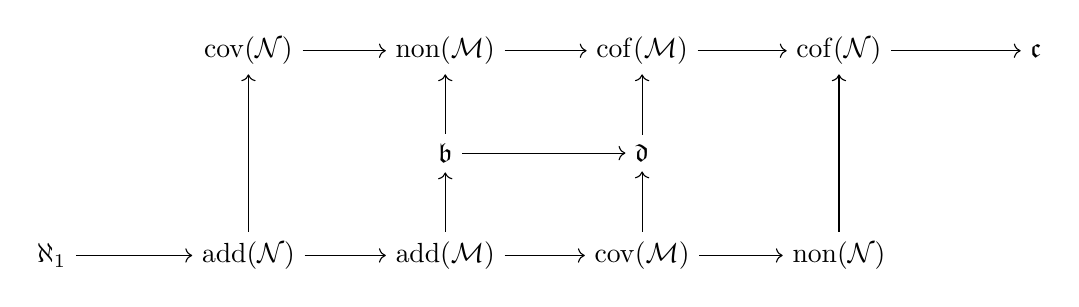
\begin{tikzpicture}
		\newcommand{\w}{2.5}
		\newcommand{\h}{1.3}
		
		\node (aleph1) at (-\w, 0) {$\aleph_1$};
		
		\node (addN) at (0, 0) {$\add(\nul)$};
		\node (covN) at (0, \h*2) {$\cov(\nul)$};
		
		\node (addM) at (\w, 0) {$\add(\meager)$};
		\node (b) at (\w, \h) {$\mathfrak{b}$};
		\node (nonM) at (\w, \h*2) {$\non(\meager)$};
		
		\node (covM) at (\w*2, 0) {$\cov(\meager)$};
		\node (d) at (\w*2, \h) {$\mathfrak{d}$};
		\node (cofM) at (\w*2, \h*2) {$\cof(\meager)$};
		
		\node (nonN) at (\w*3, 0) {$\non(\nul)$};
		\node (cofN) at (\w*3, \h*2) {$\cof(\nul)$};
		
		\node (c) at (\w*4, \h*2) {$\frakc$};
		
		\draw[->] (aleph1) to (addN);
		\draw[->] (addN) to (covN);
		\draw[->] (addN) to (addM);
		\draw[->] (covN) to (nonM);	
		\draw[->] (addM) to (b);
		\draw[->] (b) to (nonM);
		\draw[->] (addM) to (covM);
		\draw[->] (nonM) to (cofM);
		\draw[->] (covM) to (d);
		\draw[->] (d) to (cofM);
		\draw[->] (b) to (d);
		\draw[->] (covM) to (nonN);
		\draw[->] (cofM) to (cofN);
		\draw[->] (nonN) to (cofN);
		\draw[->] (cofN) to (c);
	\end{tikzpicture}
	\]
	ここで矢印$A \to B$は$A \le B$をZFCで証明できることを意味する.
	また$\add(\meager) = \min \{ \cov(\meager), \frakb \}$かつ$\cof(\meager) = \max \{ \non(\meager), \frakd \}$がZFCで証明できる.
	
	Cichońの図式に表示されている基数不変量以外にもBlassの図式と呼ばれる図式の基数不変量:$\mathfrak{m}, \mathfrak{p}, \mathfrak{h}, \mathfrak{g}, \mathfrak{s}, \mathfrak{e}, \mathfrak{r}, \mathfrak{a}, \mathfrak{u}, \mathfrak{i}$などもある.しかし,本稿ではこれらには焦点を当てない.
	
	\begin{table}[p]\label{table:history}
		\caption{Cichońの図式の歴史}
			\begin{tabular}{@{} l|l|p{8cm}}
			年     & 人物                                & 出来事                                                                                                                                                       \\ \hline
			1875年 & du Bois-Reymond & $\aleph_0 < \frakb$の証明 \\ \hline
			1891年 & Cantor & $\aleph_0 < \frakc$の証明 \\ \hline
			1938年 & Rothberger                        & $\cov(\meager) \le \non(\nul)$と$\cov(\nul)\le\non(\meager)$の証明                                                                                            \\ \hline
			1963年 & Cohen                             & 連続体仮説の独立性                                                                                                                                                 \\ \hline
			1970年 & Martin--Solovay                   & Martinの公理およびその帰結の$\add(\nul)=\frakc>\aleph_1$の証明                                                                                                           \\ \hline
			1977年 & Truss                             & $\min\{\cov(\meager), \frakb\} \le \add(\meager)$の証明                                                                                                       \\ \hline
			1981年 & Miller                            & $\add(\meager) \le \min\{\cov(\meager), \frakb\}$の証明およびこの時点で知られていたモデルでのCichonの図式の中の基数不変量の値の決定,Kunen-Millerの表 (5x5マス) \\ \hline
			1984年 & Miller                            & $\add(\nul) \le \frakb$の証明; Kunen-Millerの表 (6x6マス)                                                                                                        \\ \hline
			1984年 & Bartoszyński                      & $\add(\nul) \le \add(\meager)$の証明                                                                                                                         \\ \hline
			1984年 & Fremlin                      & $\cof(\meager) = \max\{\non(\meager), \frakd\}$の証明; Cichoń's diagram登場                                                                                                                     \\ \hline
			1985年 & Raisonnier--Stern                 & $\cof(\meager) \le \cof(\nul)$の証明                                                                                                                         \\ \hline
			1989年 & Bartoszyński--Judah--Shelah       & $\mathrm{PT}_{f,g}$強制法の開発および連続体濃度が$\aleph_2$のときのCichońの図式の分離すべて完成                                                 \\ \hline
			2019年 & Goldstern--Kellner--Shelah         & 巨大基数を仮定したCichoń's maximumの証明                                                                                                                              \\ \hline
			2021年 & Goldstern--Kellner--Mejía--Shelah & 巨大基数を仮定しないCichoń's maximumの証明                                                                                                                             
		\end{tabular}
	\end{table}

	表\ref{table:history}にCichońの図式の歴史をまとめた.
	
	連続体仮説の否定の無矛盾性以前にRothbergerの結果があるのがすごいが,この結果は「Luzin集合とSierpinski集合の両方が存在するならば連続体仮説が成り立つ」という定理の補題として証明された.
	Cantorの$\aleph_0 < \frakc$以前にdu Bois-Reymondが$\aleph_0 < \frakb$を示していたことも驚くべきところであろう.
	
	Kunen-Millerの表というのは図\ref{fig:kunen-miller}のようなものである.\cite{Miller1981SomePO}から抜粋した.Cichońの図式ができる前はどの組合せが可能かこのような表で表していた.
	
	\begin{figure}[p]\label{fig:kunen-miller}
		\begin{center}
		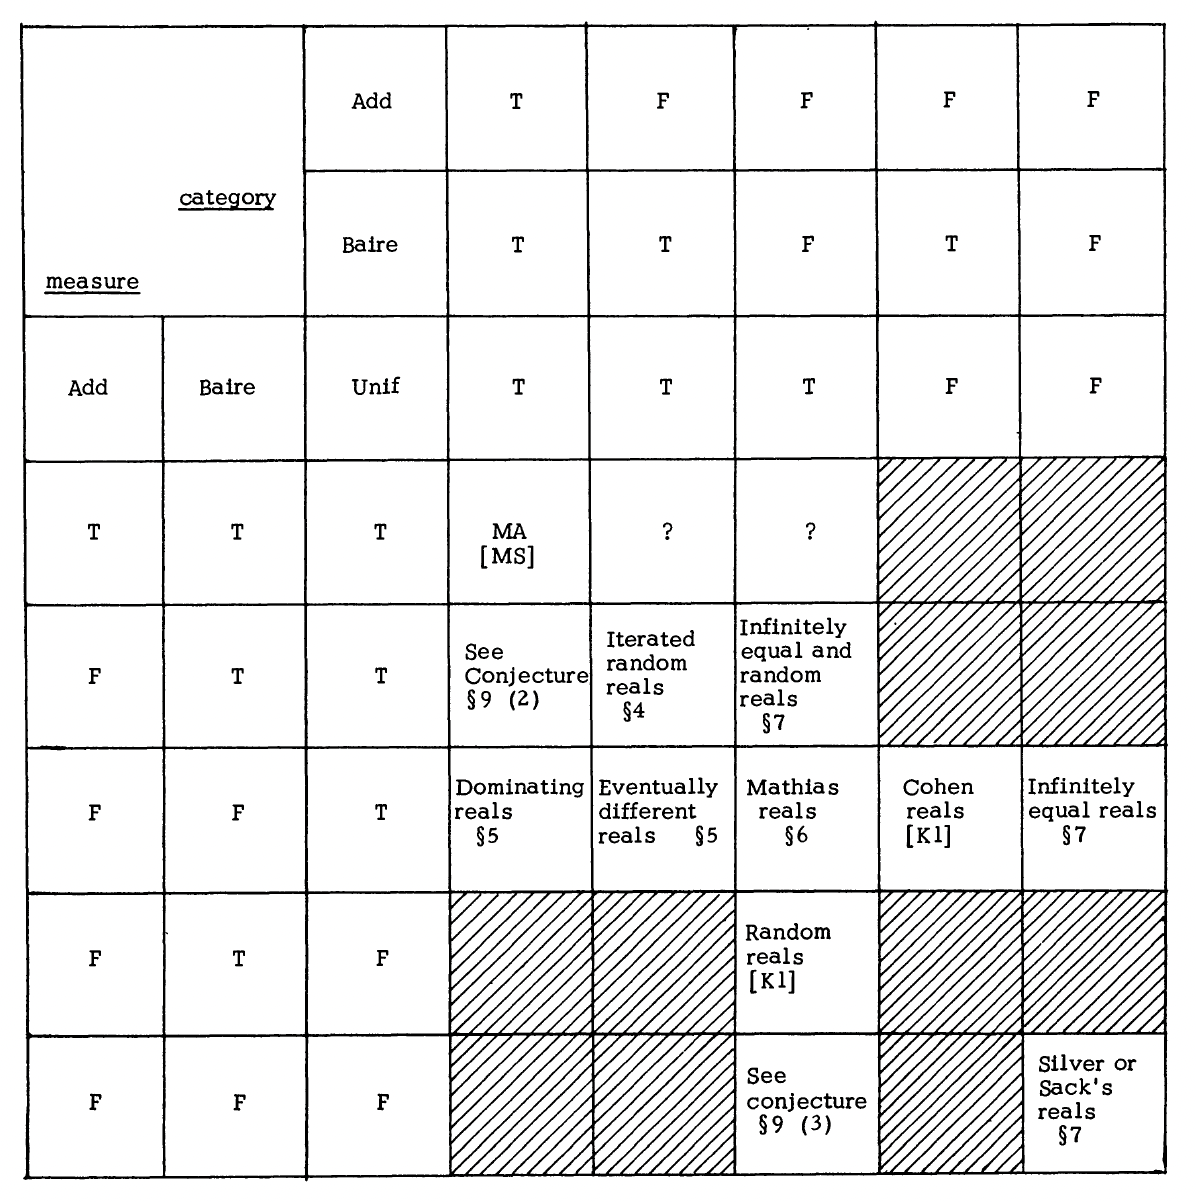
\includegraphics[width=7cm]{kunen-miller.png}
		\caption{Kunen-Millerの表}
		\end{center}
	\end{figure}
	
	表題にもなっているCichoń's maximumであるが,これはCichońの図式において (他の基数不変量の値に束縛されている$\add(\meager), \cof(\meager)$を除いて)すべての基数不変量の値を同時に別々の値にするモデルである.
	そのようなモデルの構成法を本稿では見ていく.
	
	\subsection{関係システム}
	
	\begin{defi}
		3つ組$\relR = (X, Y, \sqsubset)$が\textbf{関係システム}であるとは,$X, Y$が集合で$\sqsubset$が関係であることを言う (基本的には$\mathord{\sqsubset} \subset X \times Y$だがはみ出ていてよい).
		
		$F \subset X$が$\relR$\textbf{有界}であるとは$(\exists y \in Y)(\forall x \in F) (x \sqsubset y)$を満たすことである.
		$E \subset Y$が$\relR$\textbf{-dominanting}であるとは$(\forall x \in X)(\exists y \in E) (x \sqsubset y)$を満たすことである.
		
		\begin{itemize}
			\item $\frakb_\relR = \min \{ \abs{F} :  F \subset X \text{は}\relR\text{非有界} \}$
			\item $\frakd_\relR = \min \{ \abs{E} :  E \subset Y \text{は}\relR\text{-dominating} \}$
		\end{itemize}
		と定める.
	\end{defi}

	\begin{defi}
		関係システム$\relR = (X, Y, \sqsubset)$についてその双対を$\relR^\perp = (Y, X, \sqsubset^\perp)$と定める.ここに
		\[
		y \sqsubset^\perp x \iff \neg (x \sqsubset y).
		\]
	\end{defi}

	$\frakb_{\relR^\perp} = \frakd_\relR$かつ$\frakd_{\relR^\perp} = \frakb_\relR$に注意する.
	
	\begin{defi}
		関係システム$\relR = (X, Y, \sqsubset)$が\textbf{ポーランド関係システム}であるとは,次の3条件を満たすことを言う.
		\begin{enumerate}
			\item $X$は完全ポーランド空間.
			\item $Y$はあるポーランド空間$Z$の非空な解析集合.
			\item $\mathord{\sqsubset} \cap (X \times Z) = \bigcup_{n \in \omega} \mathord{\sqsubset}_n$であって,$\seq{\mathord{\sqsubset}_n : n \in \omega}$は$X \times Z$の閉集合の増大列であって,各$n \in \omega$と$y \in Y$について$(\mathord{\sqsubset}_n)^y = \{x \in X : x \sqsubset_n y \}$はnowhere denseである.
		\end{enumerate}
	\end{defi}

	ポーランド関係システムのような定義可能な関係システムを考えているとき,それを書いたときには今考えている宇宙の中でその定義を解釈したものを表すことにする.

	\begin{fact}
		$\relR$がポーランド関係システムであれば,$\frakb_\relR \le \non(\meager)$かつ$\cov(\meager) \le \frakd_\relR$である.
	\end{fact}

	\begin{defi}
		\begin{enumerate}
			\item $\mathcal{C} = \{ (q_n)_{n \in \omega}	 : \text{各}q_n\text{は正の有理数かつ} \sum_n q_n \le 1 \}$とおく.
			\item $\Omega_n = \{ a \in [2^{<\omega}]^{<\aleph_0} : \mu(\bigcup_{s \in a} [s]) \le 2^{-n} \}$とおき,$\Omega = \prod_{n \in \omega} \Omega_n$とおく.各$x \in \Omega$について$N_x = \bigcap_{n \in \omega} \bigcup_{s \in x(n)} [s]$とおく.
		\end{enumerate}
	\end{defi}

	以下の4つはすべてポーランド関係システムである.
	
	\begin{defi}
		\begin{enumerate}
			\item $\relR_1 = (\mathcal{C}, \mathcal{C}, \{(x,y) : (\forall^\infty n) (x(n) \le y(n))\})$
			\item $\relR_2 = (\Omega, 2^\omega, \{ (x, y) : y \not \in N_x \})$
			\item $\relR_3 = (\omega^\omega, \omega^\omega, \{ (x,y) : (\forall^\infty n)(x(n) \le y(n))\})$
			\item $\relR_4 = (\omega^\omega, \omega^\omega, \{ (x,y) : (\forall^\infty n)(x(n) \ne y(n)) \})$
		\end{enumerate}
	\end{defi}

	\begin{lem}
		\begin{enumerate}
			\item $\frakd_{\relR_1} = \cof(\nul), \frakb_{\relR_1} = \add(\nul)$,
			\item $\frakd_{\relR_2} = \non(\nul), \frakb_{\relR_2} = \cov(\nul)$,
			\item $\frakd_{\relR_3} = \frakd, \frakb_{\relR_3} = \frakb$,
			\item $\frakd_{\relR_4} = \cov(\meager), \frakb_{\relR_4} = \non(\meager)$.
		\end{enumerate}
	\end{lem}
	
	\subsection{Cohen,ランダム,Hechler,アメーバ,eventually different強制法}
	
		\subsubsection{Cohen強制法}
		
		$\C = 2^{<\omega}$で順序を延長関係で入れたもの$q \le p \iff p \subset q$はCohen強制法と呼ばれる.
		$\C$ジェネリックフィルター$G$から作られる実数$c = \bigcup G$をCohen実数という.
		Cohen実数から$G$を復元できる:$G = \{ c \upharpoonright n : n \in \omega \}$.
		Cohen強制法は可算なので,明らかに$\sigma$-centeredを満たす.特にcccを満たす.
		Cohen実数は$\relR_4^\perp$を解決する:
		\[
		(\forall x \in \omega^\omega \cap V)(\exists^\infty n)(x(n) = \dot{c}(n)).
		\]
		
		\subsubsection{ランダム強制法}
		
		$\B = \{ T : T\text{は}2^{<\omega}\text{の部分木で}\mu([T]) > 0 \}$で順序を包含関係で入れたもの$T' \le T \iff T' \subset T$をランダム強制法という.
		$\B$ジェネリックフィルター$G$から作られる実数$r = \bigcap \{[T] : T \in G \}$をランダム実数という.
		ランダム実数から$G$を復元できる:$G = \{ T \in \B : r \in [T] \}$.
		ランダム強制法はcccを満たす.
		ランダム実数は$\relR_2$を解決する:
		\[
		(\forall x \in \Omega^V)(\dot{r} \not \in N_x).
		\]
		
		\subsubsection{Hechler強制法}
		
		$\mathbb{D} = \{ (n, f) : n \in \omega, f \in \omega^\omega \}$で順序を
		\[(m, g) \le (n, f) \iff n \le m \land f \upharpoonright n = g \upharpoonright n \land (\forall k \in \omega)(f(k) \le g(k))\]
		で入れたものをHechler強制法という.
		$\mathbb{D}$ジェネリックフィルター$G$から作られる実数$d = \bigcup \{ f \upharpoonright n : (n, f) \in G \}$をHechler実数という.
		Hechler実数から$G$を復元できる:$G = \{ (n, f) : f \upharpoonright n = d \upharpoonright n \}$.
		Hechler強制法は$\sigma$-centeredである.
		Hechler実数は$\relR_3$を解決する:
		\[
		(\forall x \in \omega^\omega \cap V)(\forall^\infty n)(x \le^* \dot{d}).
		\]
		
		\subsubsection{アメーバ強制法}
		
		$\mathbb{A} = \{ T : T\text{は}2^{<\omega}\text{のsubtreeで}\mu([T])\ge 1/2 \}$で順序を$T' \le T \iff T' \subset T$で入れたものをアメーバ強制法という.
		$\mathbb{D}$ジェネリックフィルター$G$に対して測度$1/2$の閉集合$K_G = \bigcap G$が定まる.そのコード$a$をアメーバ実数という.アメーバ実数$a$から$G$を復元できる: $G = \{ T \in \mathbb{A} : \hat{a} \subset [T] \}$.
		アメーバ実数をBorelな方法で加工して得られる実数$b \in \mathcal{C}$があって,それは$\relR_1$を解決する:
		\[
		(\forall x \in \mathcal{C}^V) (x \le b).
		\]
		アメーバ強制法はcccである.
		
		\subsubsection{eventually different強制法}
		
		$\mathbb{E} = \{ (s,k,\varphi) : s \in \omega^{<\omega}, k \in \omega, \varphi \colon \omega \to [\omega]^{\le k}, (\forall i \in \dom(s))(s(i) \not \in \varphi(i)) \}$で順序を
		\[
		(s', k', \varphi') \le (s, k, \varphi) \iff s \subset s' \land k \le k' \land (\forall i)(\varphi(i) \subset \varphi'(i))
		\]
		を入れたものをeventually different強制法という.	
		$\mathbb{E}$ジェネリックフィルター$G$から作られる実数$e = \bigcup \{ s  : (s, k, \varphi) \in G \}$をeventually different generic実数という.
		eventually different強制法は$\sigma$-centeredである.
		eventually different generic実数は$\relR_4$を解決する:
		\[
		(\forall x \in \omega^\omega \cap V)(\forall^\infty n)(x(n) \ne \dot{e}(n)).
		\]
		
		\subsubsection{Borel reading of names}
		
		Cohen,ランダム,Hechler,アメーバ,eventually different強制法は共通して次の性質を持つ.
		
		\begin{property}\label{property:hasgenericreal}
			$\P$をcccかつBorelな強制半順序であり,かつ$\P$はジェネリック実数を持つという性質を考える.
			すなわち,実数の名前$\dot{x}_\mathrm{gen}$とBorelな関係$B \subset \P \times 2^\omega$があって
			\[
			\P \forces p \in \dot{G} \iff B(p, \dot{x}_\mathrm{gen})
			\]
			となるという性質を考える.
		\end{property}
	
		この性質を持つ強制法による強制拡大での実数はジェネリック実数からBorelな方法で計算できる.
		\begin{prop}
			$\P$を上記性質\ref{property:hasgenericreal}を持つ強制法とする.
			$\dot{x}$を$2^\omega$の元の名前とする.
			このときBorel関数$C \colon 2^\omega \to 2^\omega$があって,
			\[
			\forces \dot{x} = C(\dot{x}_\mathrm{gen})
			\]
			となる.
		\end{prop}
	
		これは有限台反復でも同様である.
		\begin{prop}
		$(P_\alpha, Q_\alpha : \alpha < \delta)$を有限台反復とする.
		各$Q_\alpha$は上記性質\ref{property:hasgenericreal}を持つ(ことが$P_\alpha$によって強制される)強制法とする.
		$\dot{x}$を$2^\omega$の元の$P_\delta$名前とする.
		このときBorel関数$C \colon (2^\omega)^\omega \to 2^\omega$と可算個の添字$\alpha_0, \alpha_1, \dots$があって,
		\[
		\forces \dot{x} = C(\dot{x}_\mathrm{gen}^{\alpha_0}, \dot{x}_\mathrm{gen}^{\alpha_1}, \dots)
		\]
		となる.
		\end{prop}
		
	\subsection{goodness}
	
	\begin{defi}
		$P$をcccな強制法とし,$\lambda$を非可算正則基数とし,$R$をポーランド関係システムとする.
		$P$が\textbf{$\lambda$-$\relR$-good}であるとは,$Y$の元を表す各$P$名称$\dot{y}$について非空な集合$\mathscr{Y} \subset Y$でサイズ$<\lambda$なものが$V$に存在して,どんな$x \in X$についても$x$が$\mathscr{Y}$上$\relR$非有界であれば,$\forces x \not \sqsubset \dot{y}$.
	\end{defi}

	\begin{fact}
		$\relR$をポーランド関係システムとする.
		\begin{enumerate}
			\item cccでサイズ$< \lambda$な強制法$P$はすべて,$\lambda$-$\relR$-goodである.特にCohen強制法は$\aleph_1$-$\relR$-goodである.
			\item cccで$\lambda$-$\R$-goodであることは任意の長さの有限台反復で保たれる.
		\end{enumerate}
	\end{fact}

	\begin{fact}
	\begin{enumerate}
		\item $\sigma$-centeredかランダム強制法の部分ブール代数である強制法は$\aleph_1$-$\relR_1$-goodである.
		\item $\sigma$-centeredな強制法は$\aleph_1$-$\relR_2$-goodである.
	\end{enumerate}
	\end{fact}

	\begin{lem}
		$\relR = (X, Y, \sqsubset)$をポーランド関係システムとする.
		$\lambda \le \kappa \le \mu$を全て非可算正則基数とする.
		$\mu$個のCohen実数$(c_\alpha : \alpha < \mu)$を加えた後に,$\lambda$-$\relR$-good強制法で強制拡大したモデルにおいて,どんな実数$y \in Y$についても,
		\[
		(\exists \alpha < \kappa)(\forall \beta \in \kappa \setminus \alpha)(c_\beta \not \sqsubset y)
		\]
		が成り立つ.
	\end{lem}
	\begin{proof}
		$\kappa$個のCohen実数を追加した後の中間モデルで議論する.それを$V_\kappa$と呼ぶ.
		残りの強制法,すなわち$\mu\setminus\kappa$個のCohenとgood強制法の反復はgoodである.
		よって$V_\kappa$においてgoodnessを目撃する集合$\mathcal{Y}$でサイズ${<}\lambda$なものを得る. 

		最初のCohen強制法はcccであり,$\kappa\ge \lambda$は正則なので,ある番号$\alpha\in\kappa$がとれてどの元$y \in \mathcal{Y}$もすでに
		最初の$\alpha$個のCohenを付け加えたモデルに存在する.そのモデルを$V_{\alpha}$と書こう.
		$y$によってboundされる実数たちの集合$M_y$はmeagerであり,それは絶対的である.
		どの$\beta\in\kappa\setminus \alpha$に対しても$c_\beta$は$V_{\alpha}$上のCohen実数なので$M_y$に属さない.すなわち$y$にboundされない.
		つまり,$\mathcal Y$によってboundされない.
		したがって,goodnessの定義より,各$c_\beta$は与えられた$y$にboundされないことが強制される.
	\end{proof}
	
	\subsection{$\EUB$と$\COB$}
	
	\begin{defi}
		$\gamma$を極限順序数,$P$をccc強制法,$\relR = (X, Y, \sqsubset)$を定義可能な関係システムとする.
		$\EUB(\relR, P, \gamma)$とは次の主張である:
		$X$の元の$P$-名称の列$(\dot{x}_\alpha)_{\alpha < \gamma}$であって,どんな$Y$の元の$P$-名称の列$\dot{y}$についても
		\[
		(\exists \alpha < \gamma)(\forall \beta \in \gamma \setminus \alpha)\ P \forces \neg (\dot{x}_\beta \sqsubset \dot{y})
		\]
		となる.
	\end{defi}
	ccc強制法を考えているので,$\gamma$が非可算共終数を持つときには,$(\exists \alpha < \gamma)(\forall \beta \in \gamma \setminus \alpha)$は強制関係の外にあろうが中にあろうが同じなことに注意しておく.
	
	\begin{defi}
		$\lambda, \mu$を非可算正則基数,$P$をccc強制法,$\relR = (X, Y, \sqsubset)$を定義可能な関係システムとする.
		このとき$\COB(\relR, P, \lambda, \mu)$は次の主張である:
		${<}\lambda$-directedな半順序集合集合$(S, \prec)$でサイズ$\mu$なものと$Y$の元の$P$-名称の族$(\dot{y}_s : s \in S)$があって,$X$の元のどんな$P$-名称$\dot{x}$についても
		\[
		(\exists s \in S)(\forall t \succ s) \ P \forces \dot{x} \sqsubset \dot{y}_i
		\]
		となる.
	\end{defi}

	$\EUB(\relR, P, \gamma)$は$\COB(\relR, P, \cf(\gamma), \cf(\gamma))$と同値なことに注意する.
	
	\begin{lem}\label{lem:cobimpliesineq}
		$\COB(\relR, P, \lambda, \mu)$は$P \forces (\frakb_\relR \ge \lambda \AND \frakd_\relR \le \mu)$を含意する.
	\end{lem}
	\begin{proof}
		集合$(\dot{y}_s)_{s\in S}$はサイズ$\mu$のdominating familyなので$\mathfrak{d}_\relR\le \mu$を得る.

		$\mathfrak{b}_\relR \ge \lambda$を示すために,$(\dot{x}_\alpha)_{\alpha\in\theta}$を長さ$\theta<\lambda$なる$X$の元の$P$名前の列とする.
		各$\dot{x}_\alpha$について,$s_\alpha\in S$があって,$(\forall t\succ s_\alpha)\, P\forces \dot{x}_\alpha \sqsubset \dot{y}_t$である.
		$S$は${<}\lambda$-directedなので,ある$t$があってどの$s_\alpha$よりも大きい.
		したがって,$P\forces \dot{x}_\alpha \sqsubset \dot{y}_t $がすべての$\alpha$で成り立つ.
		すなわち$\{\dot{x}_\alpha:\, \alpha\in\theta\}$はboundedである.
	\end{proof}

	上の注意と補題\ref{lem:cobimpliesineq}より$\EUB(\relR, P, \lambda)$は$P \forces (\frakb_\relR \le \lambda \AND \frakd_\relR \ge \lambda)$を含意する.
	
	\section{Cichońの図式の左半分}
	
	\begin{assumption}\label{asm:P}
		$\aleph_1<\lambda_1<\lambda_2<\lambda_3<\lambda_4<\lambda_5$を正則基数たちで
		$\mu<\lambda_i$ならば$\mu^{\aleph_0}<\lambda_i$となるものたちとする.
		また,$\lambda_3$は正則基数$\chi$で$\chi^{\aleph_0}=\chi$なものの後続基数だと仮定し,$\lambda_5^{<\lambda_4}=\lambda_5$とする.
		
		$\delta_5=\lambda_5+\lambda_5$とおき,$\delta_5\setminus\lambda_5$の非有界部分集合たち$S^1$, $S^2$, $S^3$ and $S^4$への分割を固定する.
		各$\alpha\in \delta_5\setminus\lambda_5$ について$w_\alpha\subseteq \alpha$であって各$\{w_\alpha:\, \alpha\in S^i\}$は $[\delta_5]^{{<}\lambda_i}$の中で共終であると仮定する.
	\end{assumption}
	
	\begin{defi}\label{def:Pa}
		$\Pa=(P_\alpha,Q_\alpha)_{\alpha\in\delta_5}$ 
		を有限台反復であって,$\alpha\in \lambda_5$に対する$Q_\alpha$はCohen強制法であり
		\begin{flalign*}
			&&
			Q_\alpha\text{ は$w_\alpha$-部分的 }
			\left\{
			\begin{array}{c}
				\text{アメーバ}\\
				\text{ランダム}\\
				\text{Hechler}\\
				\text{eventually different}\\
			\end{array}\right\}
			\text{ 強制法} \hspace{0.5cm} \text{($\alpha$が}
			\left\{
			\begin{array}{l}
				S^1\\
				S^2\\
				S^3\\
				S^4\\
			\end{array}
			\right\} \text{の元のとき)}
			\\
		\end{flalign*}
		であるものとする.
	\end{defi}
	
	\section{ブール超冪}
	
	$\kappa$を強コンパクト基数とし,$B$を$\kappa$分配的かつ$\kappa^+$-ccを持つ無原子完備ブール代数とする.
	すると任意の$B$内の$\kappa$完備フィルターは$\kappa$完備なウルトラフィルターに拡大される.
	また,ある$B$の反鎖$A_0$で濃度$\kappa$なものがあって,$A_0 \cap U = \emptyset$を満たす.
	今,$\kappa$完備なウルトラフィルター$U$を固定する.
	
	\textbf{BUP名前}とは関数$x \colon A \to V$であって,その定義域$A$は$B$の極大反鎖であるものである.
	$x$の定義域を$A(x)$と書く.
	
	任意のBUP名前は$V$の元の$B$-名前を定める:BUP名前$x$に対して$\{ (\widecheck{x(a)}, a) : a \in A(x) \}$である.
	逆に$V$の元の$B$-名前はそれと強制同値なBUP名前を持つ.
	BUP名前とそこから定まる$B$-名前を同一視する.
	
	2つのBUP名前に対してブール値$\truth{x=y}$が定まる.$x$と$y$が同値とは$\truth{x=y} \in U$であることを指す.
	
	$v \in V$の標準名前$\check{v}$とは$\{ (1_B, v) \}$のことである.
	
	ブール超冪$M^-$はBUP名前$x$の同値類$[x]$からなる.
	$[x] \in^- [y]$を$\truth{x \in y} \in U$により定義する.
	$j^- \colon V \to M^-$を$v$を$[\check{v}]$で定める.
	
	
	
	
	\nocite{*}
	\printbibliography[title={参考文献}]
\end{document}